%\section{Backgorund information}

This chapter provides background information that is important in this research.
First, two of the most popular overlay networks used in Kubernetes are explained in detail.
Then the author explains how to utilize multi-core CPUs for packet processing in Linux.
Finally, the author explains ipvs load balancer and two of its operation modes.

\section{Overlay network}

\subsection{Network of a container}

There are several types of container network including, veth, MACVLAN, IPVLAN, host network, openvswitch.
There are good reviews of these network in \cite{Marmol2015,claassen2016linux,struye2017assessing}.
The author uses the container network that uses veth because of the popularity and easiness of the setups.
Here the setup used in the experiments is explained.

Figure~\ref{fig:bridge+veth} shows a schematic diagram of the container network used in this study.
The veth kernel module creates a pair of network interfaces that act like a pipe.
One of the peer interfaces is kept in the host network namespace and the other is added to the container namespace.
The interface on the host network namespace is added to a network bridge.
In the case of Docker, most of the veth setup is done by the Docker daemon.

The communication between two containers on the same physical node is through the docker0.
The communication with the outside of the node follows the routing rules in the kernel, and optionally iptables Masquerade.  

\begin{figure}[h]
  \centering
  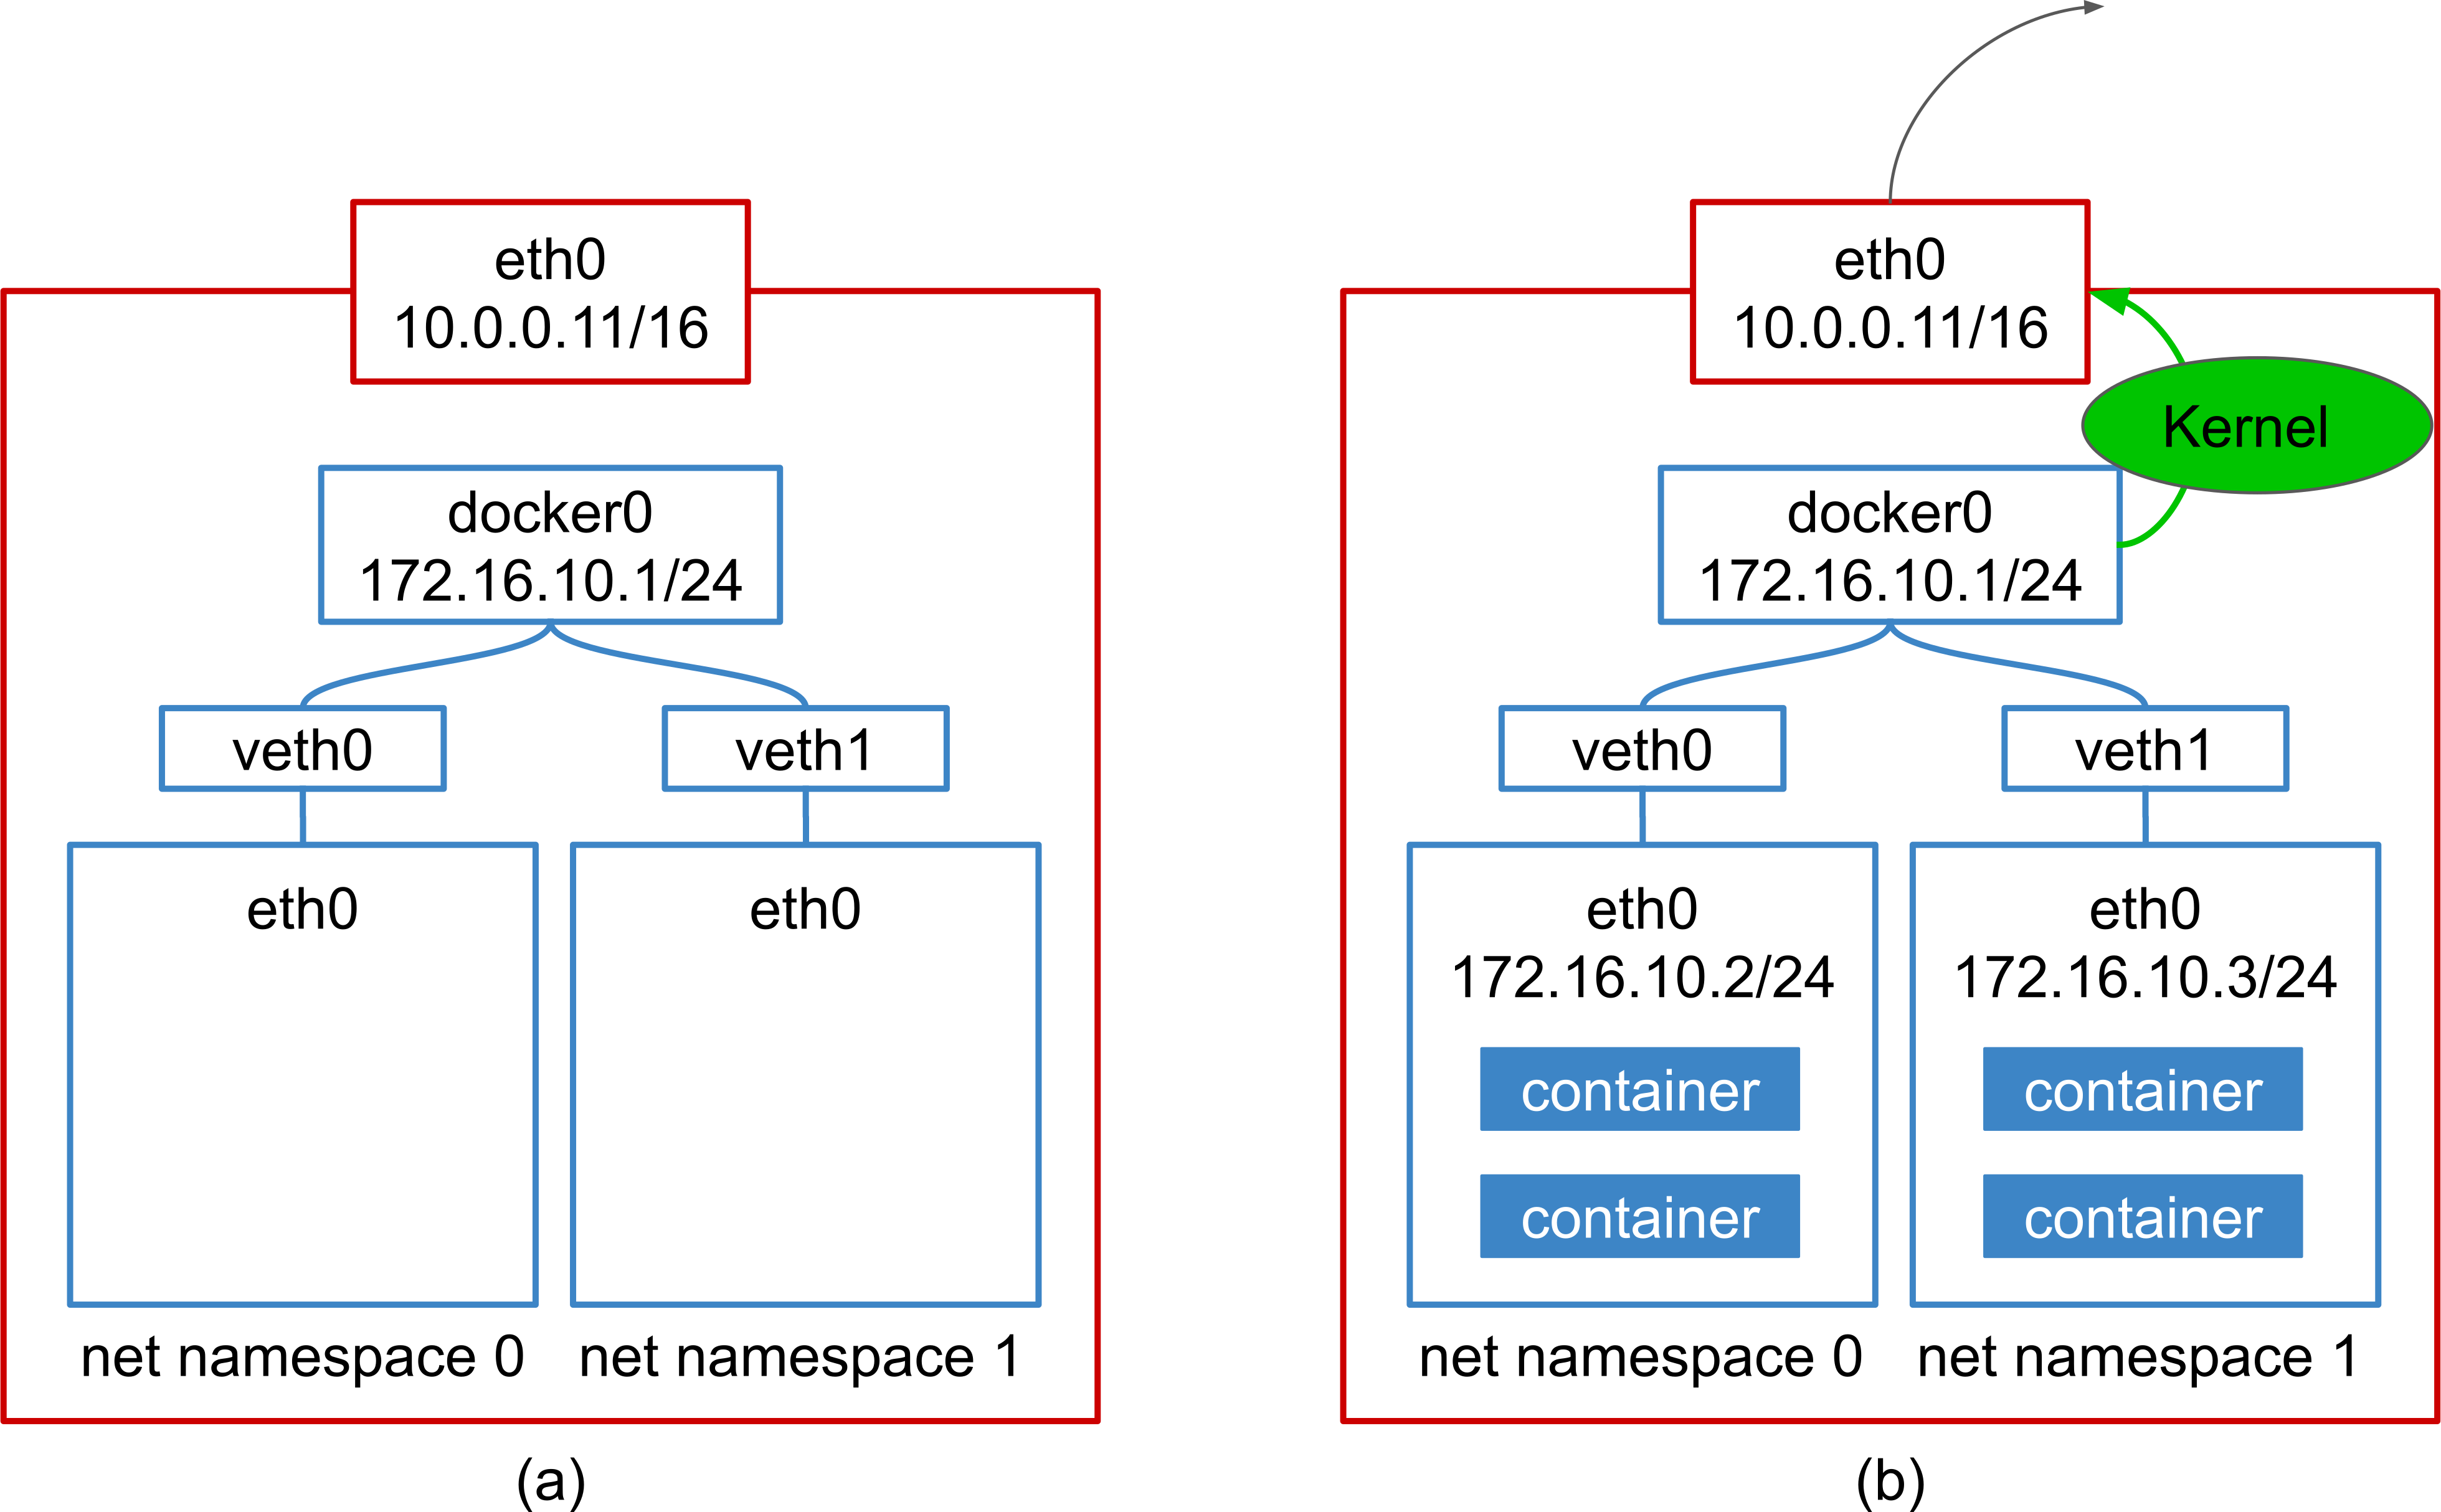
\includegraphics[width=0.8\columnwidth]{Figs/bridge+veth}

  \par\bigskip
  \centering
  \begin{minipage}{0.9\columnwidth}
    \caption[Docker networks setup]{
      Docker networks setup
    }
    \label{fig:bridge+veth}
  \end{minipage}
\end{figure}
 
When a container needs to communicate with other containers on different nodes, the kernel needs to know on which node the peer container exists.
The kernel normally does not know this, but with the help of overlay network, the kernel eventually finds out the next hop towards peer container.

\FloatBarrier

\subsection{Overlay Network}

\subsubsection{Flannel}

The author used flannel to build the Kubernetes cluster used in the experiment.
Flannel has three types of backend, {\it i.e.}, operating modes, named host-gw, vxlan, and udp\cite{CoreOSFlannelBackend}.

\subsubsection{host-gw mode}

In the host-gw mode, the flanneld installed on a node simply configures the routing table 
based on the IP address assignment information of the overlay network, which is stored in the etcd. 
When a {\em pod} on a node sends out an IP packet to {\em pods} on the different node, 
the former node consults the routing table and learn that the IP packet should be sent out to the latter.
Then, the former node forms Ethernet frames containing the destination MAC address of the latter node 
without changing the IP header, and send them out.
Since packets are not encapsulated in the host-gw mode, the MTU size remains 1500 bytes.

\begin{figure}[h]
  \centering
  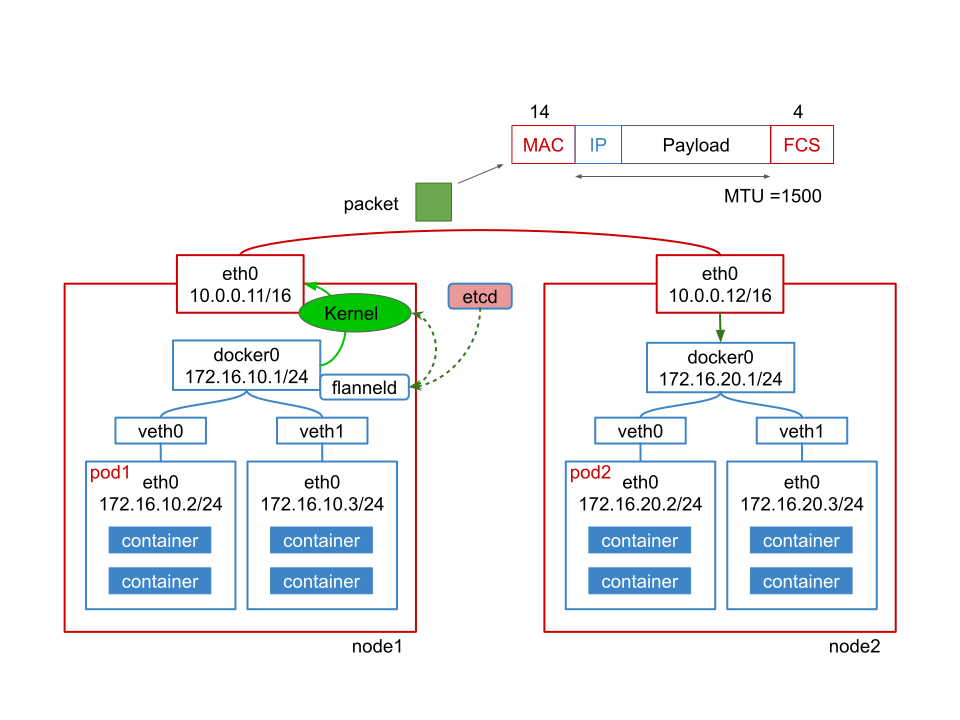
\includegraphics[width=0.8\columnwidth]{Figs/flannel-host-gw}

  \par\bigskip
  \centering
  \begin{minipage}{0.9\columnwidth}
    \caption[Flannel setup with host-gw]{
      Flannel setup with host-gw.
    }
    \label{Figs/flannel-host-gw}
  \end{minipage}
\end{figure}

\subsubsection{vxlan mode}

In the case of the vxlan mode, flanneld creates the Linux kernel's vxlan device, flannel.1. 
Flanneld will also configures the routing table appropriately based on the information stored in the etcd.
When {\em pods} on different nodes need to communicate, the packet is routed to flannel.1.
The vxlan functionality of the Linux kernel identify the MAC address of flannel.1 device on the destination node,
then form an Ethernet frame toward the MAC address.
The vxlan then encapsulates the Ethernet frame in a UDP/IP packet with a vxlan header, after which the IP packet is eventually sent out.
An additional 50 bytes of header is used in the vxlan mode, thereby resulting in an MTU size of 1450 bytes.

\begin{figure}[h]
  \centering
  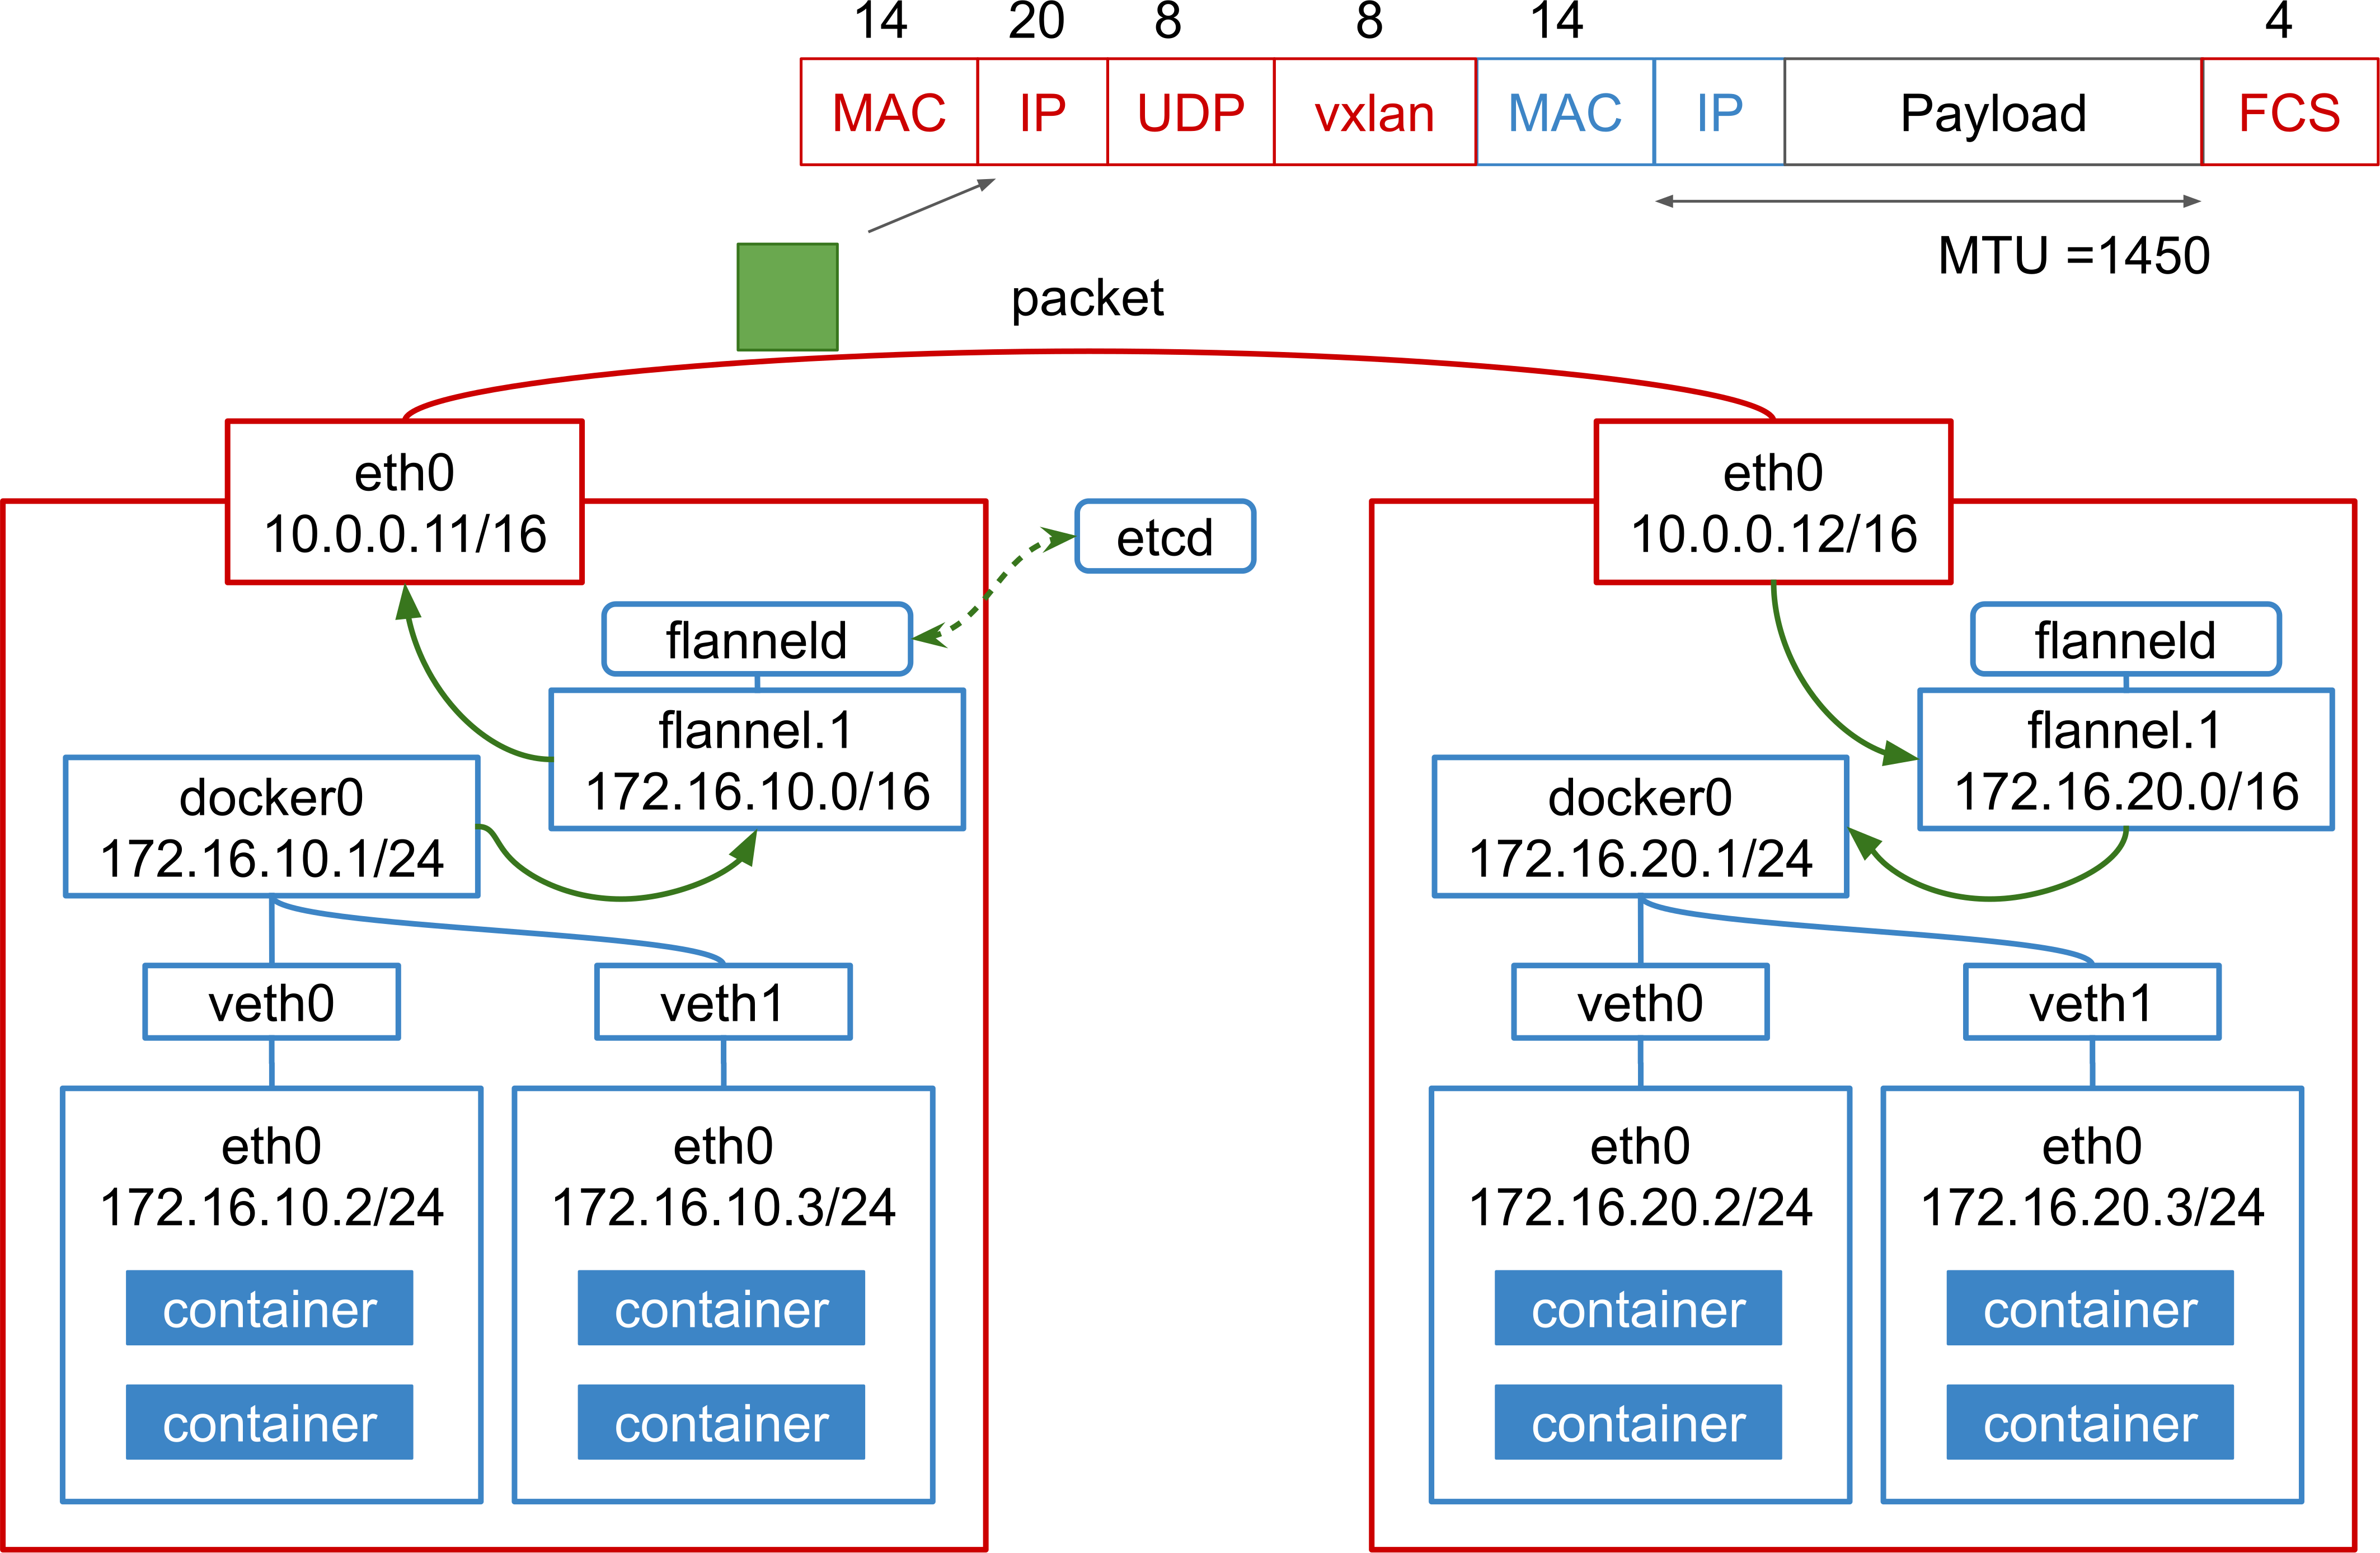
\includegraphics[width=0.8\columnwidth]{Figs/flannel-vxlan}

  \par\bigskip
  \centering
  \begin{minipage}{0.9\columnwidth}
    \caption[Flannel setup with vxlan]{
      Flannel setup with vxlan.
    }
    \label{Figs/flannel-vxlan}
  \end{minipage}
\end{figure}

\subsubsection{udp mode}

In the case of udp mode, flanneld creates the tun device, flannel0, and configures the routing table.
The flannel0 device is connected to the flanneld daemon itself.
An IP packet routed to flannel0 is encapsulated by flanneld, and eventually sent out 
to the appropriate node. 
The encapsulation is done for IP packets.
In the case of the udp mode, only 28 bytes of header are used for encapsulation, which results in an MTU size of 1472 bytes.

\begin{figure}[h]
  \centering
  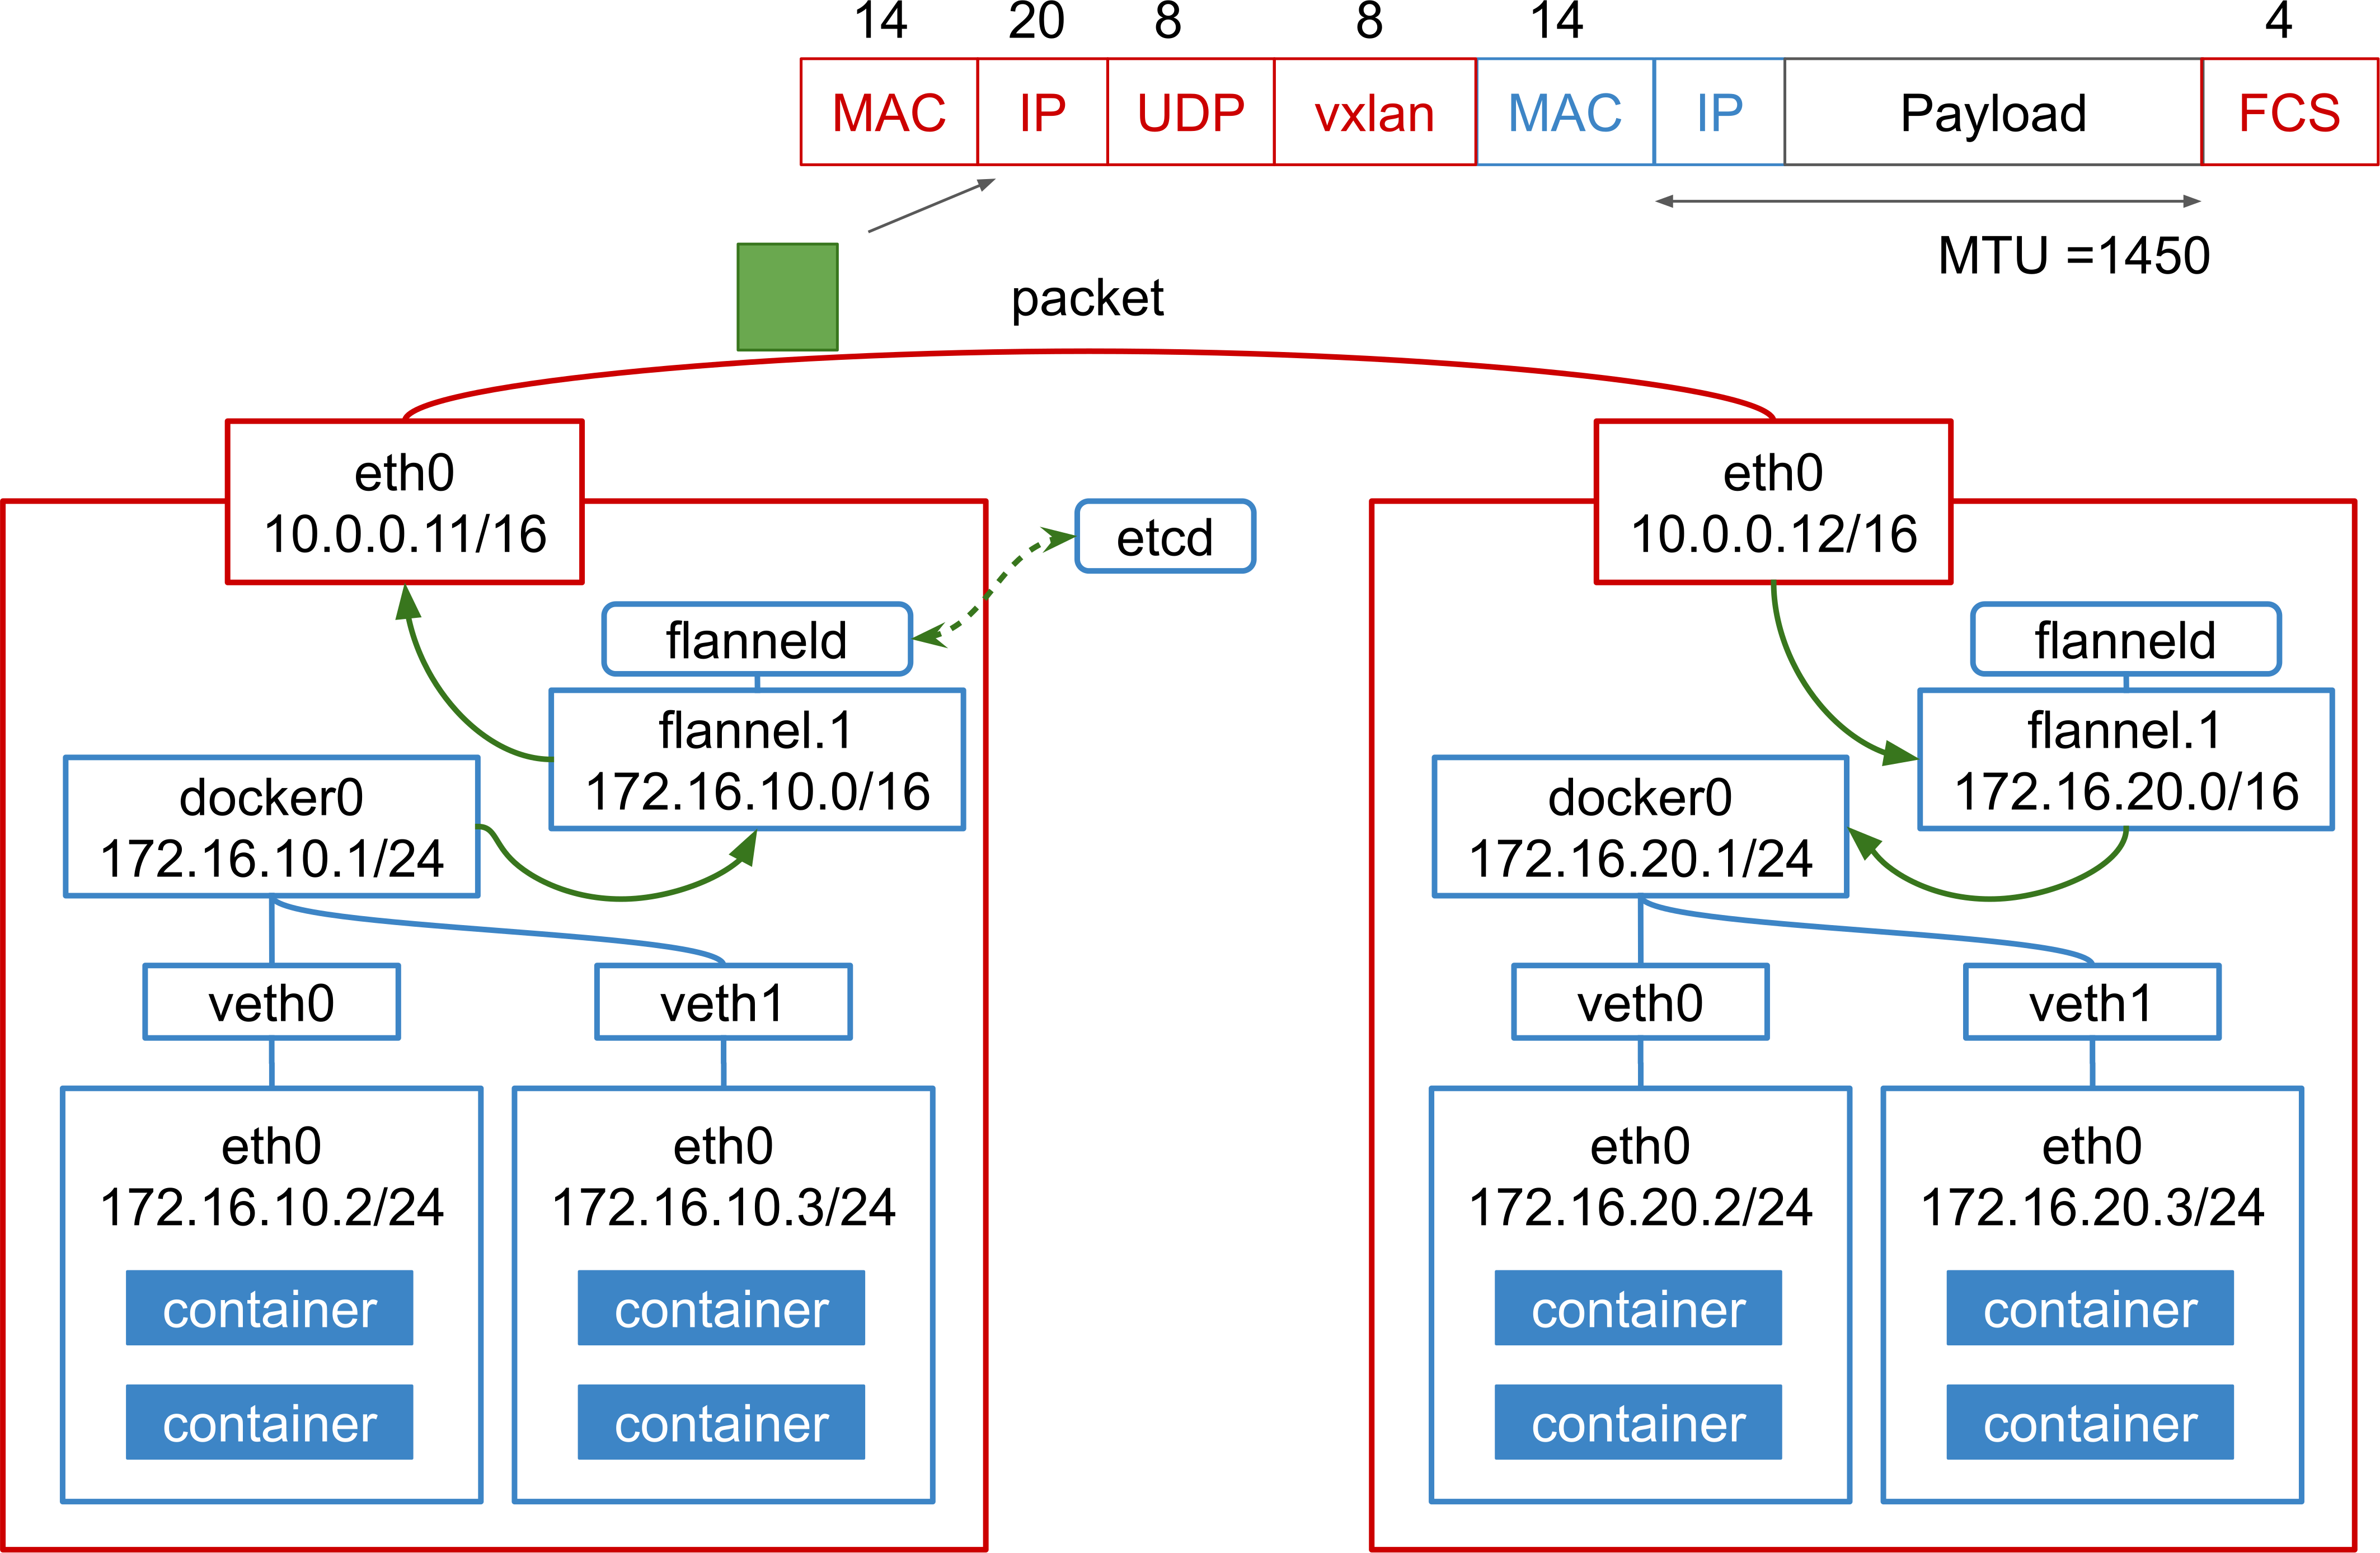
\includegraphics[width=0.8\columnwidth]{Figs/flannel-vxlan}

  \par\bigskip
  \centering
  \begin{minipage}{0.9\columnwidth}
    \caption[Flannel setup with vxlan]{
      Flannel setup with vxlan.
    }
    \label{Figs/flannel-vxlan}
  \end{minipage}
\end{figure}

\FloatBarrier

\subsection{Caveats of the overlay network}

There are caveats in using overlay network.
The author explains two of them that are identified in the course of this study.

\subsubsection{Overlay network and cloud}

Although the host-gw mode is expected to be most efficient since no packet encapsulation is used, it has a significant drawback that prohibit it to work correctly in cloud platforms. 
The host-gw mode simply sends out a packet without encapsulation.
If there is a cloud gateway between nodes, the gateway cannot identify the proper destination, thus drop the packet.

\begin{table}
  \centering
  \begin{tabular}{lccc}
    \toprule
    mode & On-premise & GCP & AWS \\
    \midrule
    host-gw & OK & NG & NG \\
    vxlan & OK & OK & OK \\
    udp & OK & OK & OK \\
    \bottomrule
\end{tabular}

  \caption{Viable flannel backend modes. In cloud environment tunnelig using vxlan or udp is needed.}
  \label{tab:Viable flannel backends}
\end{table}

The author conducted an investigation to determine which of the flannel backend mode would be usable on AWS, GCP, and on-premise data centers.
The results are summarized in Table~\ref{tab:Viable flannel backends}. 
In the case of GCP, an IP address of {\tt /32} is assigned to every VM host and 
every communication between VMs goes through GCP's gateway.
As for AWS, the VMs within the same subnet communicate directly, while the VMs in different subnets communicate via the AWS's gateway.
Since the gateways do not have knowledge of the flannel overlay network, they drop the packets; thereby, 
they prohibit the use of the flannel host-gw mode in those cloud providers.  

\subsubsection{Communication with router}

\begin{figure}[h]
\centering
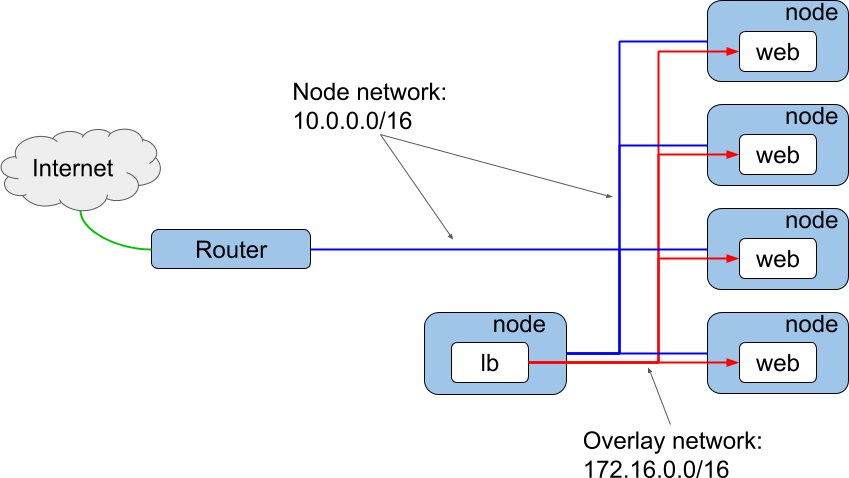
\includegraphics[width=0.8\columnwidth]{Figs/overlay.png}
\caption{The network architecture of an exemplified container cluster system. }

  A load balancer(lb) pod(the white box with "lb") and web pods are running on nodes(the blue boxes).
  The traffic from the internet are forwarded to the lb pod by the upstream router using the node network,
  and the distributed to web pods using the overlay network.

\label{fig:overlay}
\end{figure}

Fig.~\ref{fig:overlay} shows schematic diagram of network architecture of a container cluster system. 
There is a physical network(node network) with IP address range of 10.0.0.0/16 and an overlay network with IP address range of 172.16.0.0/16.
The node network is the network for nodes to communicate with each other.
The overlay network is the network setups for containers to communicate with each other.
An overlay network typically consists of appropriate routing tables on nodes, and optionally of tunneling setup using ipip or vxlan.
The upstream router usually belongs to the node network.
When a container in the Fig.~\ref{fig:overlay} communicates with any of the nodes, it can use its IP address in 172.16.0.0/16 IP range as a source IP, since every node has proper routing table for the overlay network.
When a container communicates with the upstream router that does not have routing information regarding the overlay network, the source IP address must be translated by Source Network Address Translation(SNAT) rules on the node the container resides.

\FloatBarrier
\section{Multicore Packet Proccessing}

Recently, the performance of CPUs are improved significantly due to the development of multi-core CPUs.
One of the top of the line server processors from Intel now includes up to 28 cores in a single CPU.
In order to enjoy the benefits of multi-core CPUs in communication performance, 
it is necessary to distribute the handling of interrupts from the NIC and the IP protocol processing to the available physical cores.

\begin{figure}[h]
  \centering
  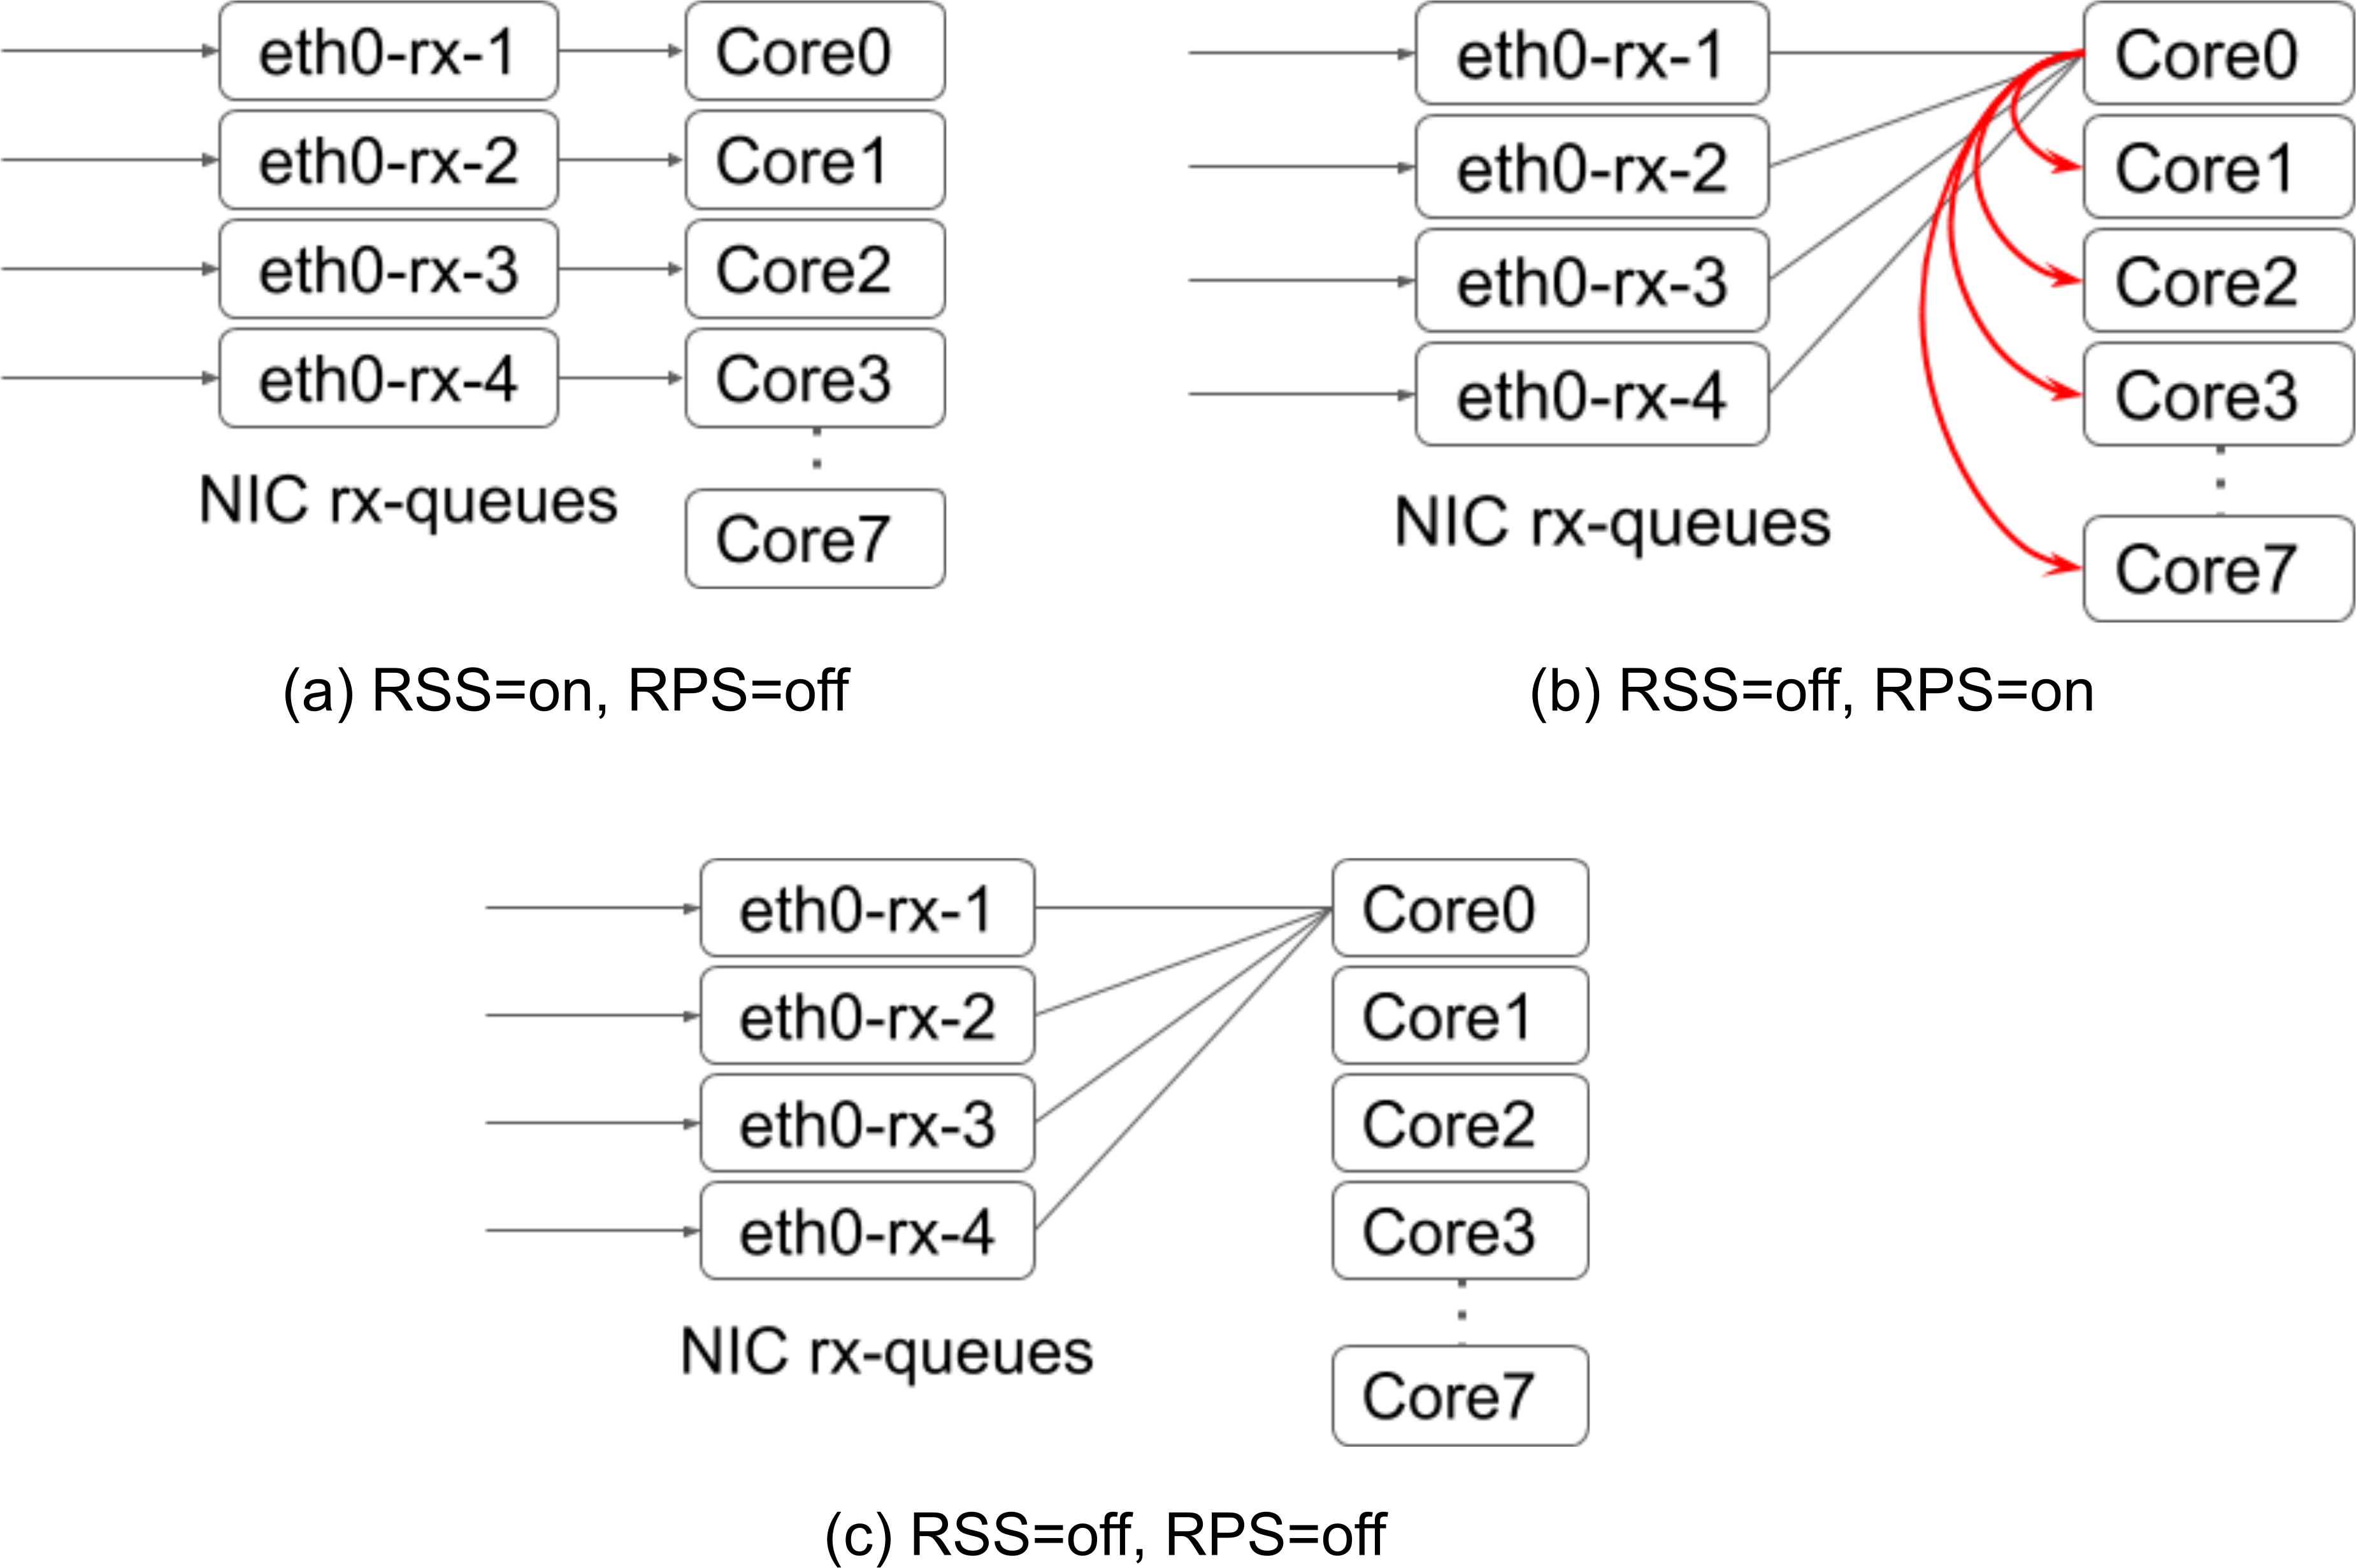
\includegraphics[width=0.8\columnwidth]{Figs/rss-rps-none}

  \par\bigskip
  \centering
  \begin{minipage}{0.9\columnwidth}
    \caption[Multicore Packet Proccessing]{
      Multicore Packet Proccessing.
    }
    \label{Figs/rss-rps-none}
  \end{minipage}
\end{figure}

%\subsubsection{RSS}
Figure~\ref{Figs/rss-rps-none} shows a schematic diagram to explain multicore packet processing of the linux system.
Receive Side Scaling (RSS)\cite{TomHerbert} is a technology 
to distribute handling of the interrupt from NIC queues to multiple CPU cores.
Subsequently, Receive Packet Steering (RPS)\cite{TomHerbert} distributes the IP protocol processing 
to multiple CPU cores by issuing inter core software interrupts.

Since load balancer performance levels could be affected by these technologies,
The author conducted an experiment to determine how load balancer performance level change depending on the RSS and RPS settings in Chapter~\ref{chapter:Performance Evaluation}.
The following shows how RSS and RPS are enabled and disabled in the experiment. 
The NIC used in the experiment is Broadcom BCM5720, which has four rx-queues and one tx-queue.
Figure~\ref{fig:rx-queue} shows the interrupt request (IRQ) number assignments to those NIC queues.

\begin{figure}
\centering
\begin{minipage}{0.5\columnwidth}
\begin{verbatim}
81: eth0-tx-0
82: eth0-rx-1
83: eth0-rx-2
84: eth0-rx-3
85: eth0-rx-4
# obtained from /proc/interrupts 
\end{verbatim}
\end{minipage}
\caption{RX/TX queues of the hardware}
\label{fig:rx-queue}
\end{figure}

When packets arrive, they are distributed to these rx-queues depending on the flow each packet belongs to.
Each receive queue has a separate IRQ associated with it. The NIC triggers
this to notify a CPU when new packets arrive on the given queue.
Then, the notified CPU handles the interrupt, and performs the protocol processing. 
According to the \cite{TomHerbert}, the CPU cores allowed to be notified is controlled by setting 
a hexadecimal value corresponding to the bit maps indicating the allowed CPU cores in \enquote{/proc/irq/\$irq\_number /smp\_affinity}.
%
For example, in order to route the interrupt for eth0-rx-1 to CPU0, 
one should set \enquote{/proc/irq/82/smp\_affinity} 
to binary number {\tt 0001}, which is 1 in hexadecimal value.
Further, in order to route the interrupt for eth0-rx-2 to CPU1, one 
should set \enquote{/proc/irq/83/smp\_affinity} 
to binary number {\tt 0010}, which is 2 in hexadecimal value.

The author refer the setting to distribute interrupts from four rx-queues to CPU0, CPU1, CPU2 and CPU3 as {\tt RSS = on}. 
It is configured as the following setting: 

\begin{center}
\begin{minipage}{0.6\columnwidth}
\begin{Verbatim}[commandchars=\\\{\}]

\underline{\textbf{RSS=on}}
echo 1 > /proc/irq/82/smp_affinity
echo 2 > /proc/irq/83/smp_affinity
echo 4 > /proc/irq/84/smp_affinity
echo 8 > /proc/irq/85/smp_affinity

\end{Verbatim}
\end{minipage}
\end{center}

On the other hand, {\tt RSS = off} means that an interrupt from any rx-queue is routed to CPU0. 
It is configured as the following setting:

\begin{center}
\begin{minipage}{0.6\columnwidth}
\begin{Verbatim}[commandchars=\\\{\}]

\underline{\textbf{RSS=off}}
echo 1 > /proc/irq/82/smp_affinity
echo 1 > /proc/irq/83/smp_affinity
echo 1 > /proc/irq/84/smp_affinity
echo 1 > /proc/irq/85/smp_affinity

\end{Verbatim}
\end{minipage}
\end{center}

%\subsubsection{RPS}

The RPS distributes IP protocol processing by placing the packet
on the desired CPU's backlog queue and wakes up the CPU using inter-processor interrupts.
The author have used the following settings to enable the RPS:

\begin{center}
\begin{minipage}{0.8\columnwidth}
\begin{Verbatim}[commandchars=\\\{\}]

\underline{\textbf{RPS=on}}
echo fefe > /sys/class/net/eth0/queues/rx-0/RPS_cpus
echo fefe > /sys/class/net/eth0/queues/rx-1/RPS_cpus
echo fefe > /sys/class/net/eth0/queues/rx-2/RPS_cpus
echo fefe > /sys/class/net/eth0/queues/rx-3/RPS_cpus

\end{Verbatim}
\end{minipage}
\end{center}

Since the hexadecimal value \enquote{fefe} represented as \enquote{1111 1110 1111 1110} in binary, 
this setting will allow distributing protocol processing to all of the CPUs, except for CPU0 and CPU8.
In this paper, the author will refer this setting as {\tt RPS = on}.
%
On the other hand, {\tt RPS = off} means that no CPU is allowed for RPS. 
Here, the IP protocol processing is performed on the CPUs the initial hardware interrupt is received.
It is configured as the following settings:

\begin{center}
\begin{minipage}{0.8\columnwidth}
\begin{Verbatim}[commandchars=\\\{\}]

\underline{\textbf{RPS=off}}
echo 0 > /sys/class/net/eth0/queues/rx-0/RPS_cpus
echo 0 > /sys/class/net/eth0/queues/rx-1/RPS_cpus
echo 0 > /sys/class/net/eth0/queues/rx-2/RPS_cpus
echo 0 > /sys/class/net/eth0/queues/rx-3/RPS_cpus

\end{Verbatim}
\end{minipage}
\end{center}

The RPS is especially effective when the NIC does not have multiple receive queues or when the number of queues is 
much smaller than the number of CPU cores. 
That was the case in the experiment, where the NIC had only four rx-queues, 
while there was a CPU with eight physical cores.

\subsubsection{None}

\section{Linux vritual server}

The ipvs is a Layer-4 load balancer capability, which is included in the Linux kernel 2.6.0 released in 2003 or later, 
to distribute incoming Transmission Control Protocol(TCP) traffic to 
{\em real servers}\footnote{The term, {\em real servers} refers to worker servers that will respond to incoming traffic, 
in the original literature\cite{Zhang2000}. We will also use this term in the similar way.}\cite{Zhang2000}. 
For example, ipvs distributes incoming Hypertext Transfer Protocol(HTTP) traffic destined for a single destination IP address, 
to multiple HTTP servers(e.g. Apache HTTP or nginx) running on multiple nodes in order to improve the performance of web services.
The ipvs has three mode of operation, NAT, Tunneling and DR.
In this study the author used NAT mode and Tunneling mode.
Here the author explain them briefly.

\subsection{NAT mode}

The NAT mode works as follows: When a user accesses a virtual
service provided by the server cluster, a request packet
destined for virtual IP address (the IP address to accept
requests for virtual service) arrives at the load balancer.
The load balancer examines the packet’s destination address and port number, if they are matched for a virtual
service according to the virtual server rule table, a real
server is selected from the cluster by a scheduling algorithm, and the connection is added into the hash table
which records connections. Then, the destination address and the port of the packet are rewritten to those of
the selected server, and the packet is forwarded to the
server. When an incoming packet belongs to an established connection, the connection can be found in the
hash table and the packet will be rewritten and forwarded
to the right server. When response packets come back,
the load balancer rewrites the source address and port
of the packets to those of the virtual service. When a
connection terminates or timeouts, the connection record
will be removed in the hash table.
%
The author refers to this mode as ipvs-tun hereafter.

\subsection{Tunneling mode}

IP tunneling (IP encapsulation) is a technique to encapsulate IP datagram within IP datagram, which allows
datagrams destined for one IP address to be wrapped and
redirected to another IP address. This technique can be
used to build a virtual server that the load balancer tun-
nels the request packets to the different servers, and the
servers process the requests and return the results to the
clients directly, thus the service can still appear as a virtual service on a single IP address.

In LVS/TUN, the load balancer encapsulates
the packet within an IP datagram and forwards it to a dynamically selected server. When the server receives the
encapsulated packet, it decapsulates the packet and finds
the inside packet is destined for VIP that is on its tunnel
device, so it processes the request, and returns the result
to the user directly.
%
The author refers to this mode as ipvs-tun hereafter.

\section{Summary}


This chapter provides background information that are important in this research.
First two of the most popular overlay networks used in Kubernetes are explained in detail.
Then the author explain how to utilize multicore CPUs for packet processing in Linux.
Finally the author explain ipvs load balancer and two of its operation modes.

